\documentclass[a4,12pt]{article}
\usepackage[margin=0.5in]{geometry}
\usepackage{titlesec}
\usepackage{ifthen}
\usepackage{fancyhdr}
\usepackage{amsmath}
\usepackage{amssymb}
\usepackage{systeme}
\usepackage{amsfonts}
\usepackage[utf8]{inputenc}
\usepackage[T1]{fontenc}
\usepackage[polish,english]{babel}
\usepackage{graphicx}
\usepackage{subfig}
\usepackage{caption}

% -------- %
% SECTIONS %
% -------- %
\newcounter{problemnumber}\setcounter{problemnumber}{1}
\titlespacing\section{2pt}{5pt}{2pt}   % Spacing between Problems
\titlespacing\subsection{5pt}{10pt}{5pt} % Spacing between Parts
\newcommand{\problem}[1][-1]{
\setcounter{partnumber}{1}
\ifnum#1>0
\setcounter{problemnumber}{#1}
\fi
\section*{Problem \arabic{problemnumber}}
\stepcounter{problemnumber}
}

\newcounter{partnumber}\setcounter{partnumber}{1}
\newcommand{\ppart}[1][-1]{
\ifnum#1>0
\setcounter{partnumber}{#1}
\fi
\subsection*{Part \parttype{partnumber}}
\stepcounter{partnumber}
}

\newenvironment{question}{
%\color{gray}
\itshape
\vspace{5pt}
\begin{tabular}{|p{0.97\linewidth}}\end{tabular}\\[5pt]
}


% ------------- %
% HEADER/FOOTER %
% ------------- %
\setlength\parindent{0pt}
\setlength\headheight{30pt}
\headsep=0.50in
\pagestyle{fancy}
\lhead{\ifthenelse{\thepage=1}
{\textbf{Mikołaj Małkiński} \\ mikolaj.malkinski@est.fib.upc.edu}
{}
}
\chead{\ifthenelse{\thepage=1}
{\textbf{\huge{\hspace{60pt}HOMEWORK \hwnumber}}}
{\textbf{\large{HOMEWORK \hwnumber}}}
}
\rhead{\ifthenelse{\thepage=1}
{\textbf{{\course}} \\ \textbf{\today}}
{}
}
\cfoot{\thepage}
\renewcommand\headrulewidth{0.8pt}
\renewcommand\footrulewidth{0.8pt}



% ---------- %
% PARAMETERS %
% ---------- %
% \PARTTYPE:
% \Alph   := "Part A, Part B,  ..."
% \alph   := "Part a, Part b,  ..."
% \arabic := "Part 1, Part 2,  ..."
% \Roman  := "Part I, Part II, ..."
\newcommand\parttype{\Roman}

% \COURSE:
\newcommand\course{KMLMM}

% \HWNUMBER
\newcommand\hwnumber{PLS 2}

\newtheorem{theorem}{Theorem}

%  ------- %
% DOCUMENT %
% -------- %
\begin{document}

    \section{Introduction}

    In this work we consider a dataset of normalised handwritten digits, which were automatically scanned from envelopes by the U.S. Postal Service in 16 x 16 grayscale images.
    The total training set contains 7291 digits, however we will perform the analysis on a 5\% subset in order to assess how well tested methods perform without access to large quantities of data.
    The testing set has 2007 digits.
    The main method chosen for this work is the Partial Least Squares Regression 2 (PLS2).
    Similarly as in PCR and IBA assignments, we are dealing with a dataset of size $n$ with $X = (x_1, \ldots, x_p)$ and $Y = (y_1, \ldots, y_q)$.
    The goal is to classify images of handwritten digits from the test set, compute the error rate and compare results with previous works.

    \section{Experiments}

    To perform the Partial Least Squares Regression we use the \textit{plsr} function from R's \textit{pls} package on the training split of the dataset.
    Firstly, we choose to create 25 components and use Leave-One-Out cross-validation method.
    Then, with the help of \textit{summary}, \textit{RMSEP} and \textit{R2} functions we can analyse the details of the trained model.
    Based on Figure~\ref{fig:plsr}, which shows the values of $RMSE$ and $R^2$ depending on the number of selected components, we choose to retain 15 components.
    Then, we center the test data with respect to the mean of the training data, perform regression using selected 15 PLSR components and finally predict the class based on the max response.
    The value of $R^2_{mean}$ ($R^2$ averaged across all classes) is 0.599 and the total error rate of the model in predicting the correct handwritten digit, calculated for the testing set, is $19.38\%$.

    \begin{figure}[h!]
        \centering
        \subfloat[Root Mean Squared Error\label{fig:rmse}]{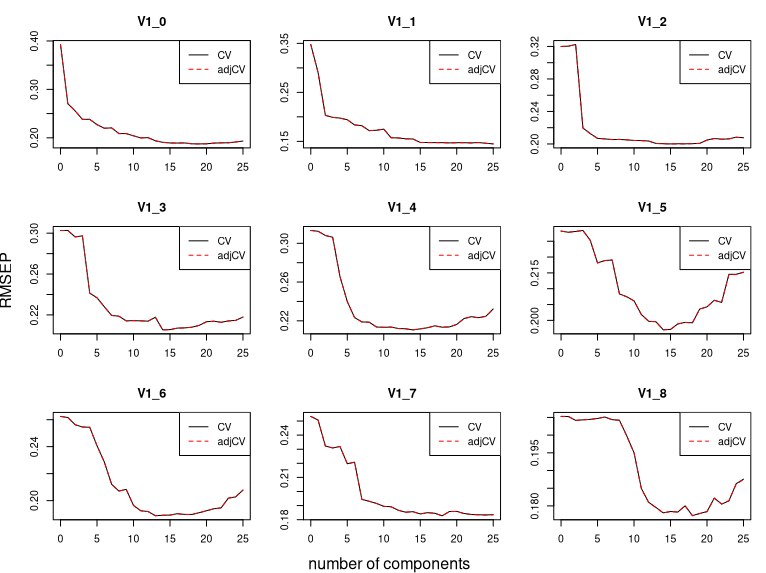
\includegraphics[width=0.5\linewidth]{rmse.png}}
        \subfloat[$R^2$\label{fig:r2}]{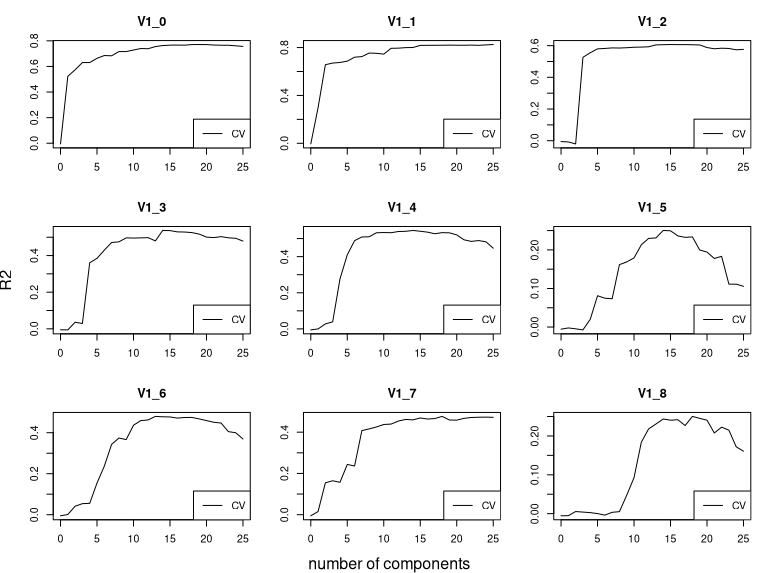
\includegraphics[width=0.5\linewidth]{r2.png}}
        \caption{
        In order to select the number of components to retain after Partial Least Squares Regression, the values of $RMSE$ and $R^2$ metrics are analysed.
        In both cases it's visible that the improvement stops after adding around the 15th component.
        Hence, for further experiments and prediction only 15 PLSR components will be used.
        }
        \label{fig:plsr}
    \end{figure}

    \section{Discussion}
    In this work an application of Partial Least Squares Regression was presented for the dataset of handwritten digits.
    When comparing the results obtained by this work to previous assignments, we can see that PLSR2 (error rate of $19.38\%$) performed better than IBA (error rate of $52.86\%$) and PCA (error rate of $38.76\%$).
    Additionally, PLSR2 required to select more components (15) than in IBA (9).

\end{document}
